\documentclass{article}

\title{Operating Systems - Notes}
\author{Harvey Hyatt}
\date{}

\usepackage[a4paper, total={7in, 10in}]{geometry}
\usepackage{graphicx}
\graphicspath{ {images/} }

\begin{document}
\maketitle

\section{Introduction}
An Operating System is a program that acts as an intermediary between a user and computer hardware. The goal is to make the system easy to use while utilizing hardware efficiently.
\begin{description}
\item[Resource Allocator] The OS manages all resources and resolves conflicting requests for resource use (e.g. allocating memory or disk space)
\item[Control System] The OS controls execution of programs to prevent errors (e.g. preventing one process from crashing another)
\end{description}
A Computer System can be divided into four components:
\begin{description}
\item[Hardware] Basic computing resources - CPU, Memory, I/O etc.
\item[Operating System] Coordinates use of hardware among processes
\item[Application Programs] Defines the way hardware resources are used to solve problems - Word processors, compilers, video games etc.
\item[Users] People, machines, other computers
\end{description}
\paragraph{Bootstrapping}
A small bootstrap program is loaded at power-up. The Firmware (BIOS) containing this program is usually stored on ROM or EEPROM. This program initializes the system - detecting connected devices and checking for memory errors - then loads the OS Kernel.
\paragraph{Computer System Organization}
\begin{center}
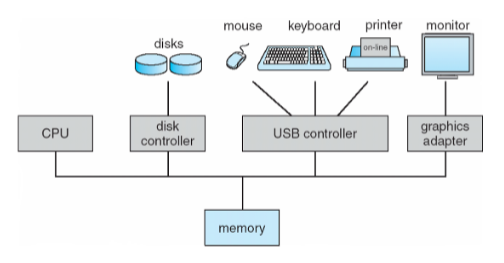
\includegraphics[scale=0.5]{fig1}
\end{center}
One or more CPUs or device controllers connect through a common bus, providing access to shared memory. CPUs and devices compete for memory cycles (i.e. to read and write memory addresses).
\paragraph{Computer System Operation} I/O devices and the CPU can execute programs concurrently. Each device controller is in charge of a particular device type, and has a local buffer (i.e. memory store for general data/control registers). The CPU moves data to/from main memory from/to controller buffers (e.g. writing data to a screen, reading coordinates from a mouse). The device controller then informs the CPU that it has finished its operation by causing an interrupt.
\paragraph{Interrupt} An interrupt transfers control to the interrupt service routine, through the interrupt vector, which contains the addresses of all the service routines. Interrupt architecture must save the address of the interrupted instruction, to resume later. Incoming interrupts are disabled while another interrupt is being processed to prevent a lost interrupt. A trap is a software-generated interrupt caused either by an error or a user request.
\paragraph{Storage Structure}
\begin{itemize}
\item Main memory - large storage media that the CPU can access directly
\item Secondary storage - extension of main memory that provides large non-volatile storage capacity
\item Magnetic disks - rigid metal or glass platters covered with magnetic recording material - surface is divided into tracks, which are divided into sectors
\item Flash memory
\end{itemize}
\paragraph{Caching} An important optimisation principle performed at many levels in the computer. Information in use is copied from slower to faster storage temporarily. The cache is checked first to determine if necessary information is there.
\paragraph{Multiprocessors} Multiprocessor systems (or parallel systems) have increased throughput and reliability. In Asymmetric Multiprocessing, CPUs have different roles, and usually one is the master of the others, while in Symmetric Multiprocessing, CPUs have identical roles, sharing process queues to service ready processes.
\paragraph{Fault Handling and Protection} A software error creates an exception or trap, which are handled as special interrupts. Other possible faults include infinite loops or processes trying to modify other process' code. Dual-mode operation allows the OS to protect itself - processes running in User Mode cannot perform privileged instructions. A system call changes the mode to Kernel, then resets to User before return. The mode bit is provided by hardware.
\paragraph{Process Management} A process is a program in execution. A Program is a passive entity while a process is an active entity. A process needs resources to accomplish its task (CPU, memory, I/O etc). Process termination requires relamation of reusable resources. A single-threaded process has one program counter, pointing to the next instruction to execute. A multi-threaded process has one program counter per thread. Concurrency is achieved by multiplexing the CPUs among the threads.
\paragraph{Process Management Activities}
\begin{itemize}
\item Creating and deleting processes
\item Suspending and resuming processes
\item Providing mechanisms for process synchronization
\item Providing mechanisms for process communication
\item Providing mechanisms for deadlock handline
\end{itemize}
\paragraph{Memory Management} All data must be in memory before and after processing, and all instructions must be in memory in order to be executed. Memory management determines what is in memory and when (avoiding excessive swapping of data between disk and memory). Memory management activities include:
\begin{itemize}
\item Keeping track of which parts of memory are currently being used and by whom
\item Deciding which processes and data to move into and out of memory
\item Allocating and deallocating memory space as needed
\end{itemize}
\paragraph{Storage Management} The OS abstracts physical properties to logical storage units (files and directories). Each medium is controlled by the respective device (e.g. CD spin speed is controlled by the disk drive). The OS manages the file system, creating and deleting files and directories, and mapping files in memory onto secondary storage.
\paragraph{I/O Subsystems} The I/O Subsystem is responsible for:
\begin{itemize}
\item Memory management of I/O (buffering - storing data temporarily while it is being transferred, caching, spooling - overlapping the output of one job with input of other jobs)
\item Abstract device-driver interface, so driver developers know how to interface their code the the OS
\item Drivers for specific hardware devices
\end{itemize}
Critical hardware such as HDDs have standardized drivers, while GPUs have more obscure ones.
\paragraph{Protection and Security}
\begin{itemize}
\item Protection - any mechanism for controlling access of processes or users to OS resources
\item Security - defense of the system against internal and external attacks
\item User IDs and Group IDs used to identify who has which privileges
\end{itemize}

\section{Architecture}

\end{document}
